\begin{frame}{What is De-featuring?}
\begin{itemize}[noitemsep,label=\textbullet,topsep=2pt,parsep=2pt,partopsep=2pt]
\item De-featuring involves removing small-irrelevant features
\item Objectives-Applications could be:
	\begin{itemize}[noitemsep,label=\textbullet,topsep=2pt,parsep=2pt,partopsep=2pt]
	\item Simplifying to reduce computation for FEM analysis
	\item Compute various levels of details (LoDs) for easier
		\begin{itemize}[noitemsep,label=\textbullet,topsep=2pt,parsep=2pt,partopsep=2pt]
		\item Graphics Rendering
		\item Data transfer via networks
		\end{itemize}
	\item Finding 'Principal' shape for
		\begin{itemize}[noitemsep,label=\textbullet,topsep=2pt,parsep=2pt,partopsep=2pt]
		\item Signature calculations for Shape Retrieval
		\item Similarity-Matching
		\item \textbf{Midsurface Computation}
		\end{itemize}
	\end{itemize}
\end{itemize}


\centering
		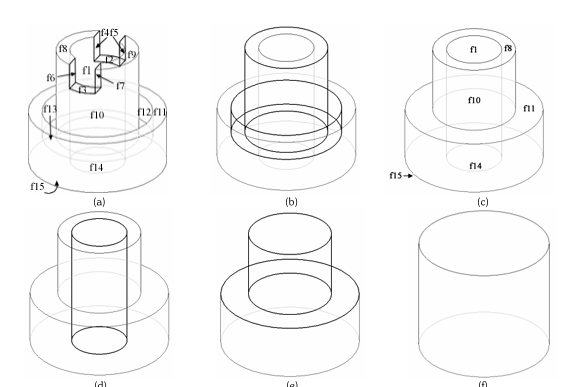
\includegraphics[width=0.25\linewidth]{..//Common/images/DefeaturingLoDs.png}


\end{frame}

\begin{frame}{How to De-feature?}
\begin{itemize}[noitemsep,label=\textbullet,topsep=2pt,parsep=2pt,partopsep=2pt]
\item Selection criterion for features depends on the domain and the context. 
\item For example, de-featuring rules for Sheet Metal Parts could be different than those of Structural parts. 
\item De-featuring rules for strength analysis could be different from those of heat-transfer analysis. These methods are in the context of preparing modeling for FEM analysis. 
\item This works uses for a different purpose - \textbf{to find the principal shape}.
\item De-featuring can be done with or without availability of ready feature information.
\item Detection and suppression becomes relatively straightforward with the ready feature-information rather than doing similar process on just the Boundary Representation (Brep).  
\end{itemize}
\end{frame}

\begin{frame}{Padmakar Dabke - Stanford}
Dabke \cite{Dabke1994} through the concept of Global Idealization was one of the first ones to leverage use of feature information for de-featuring. 

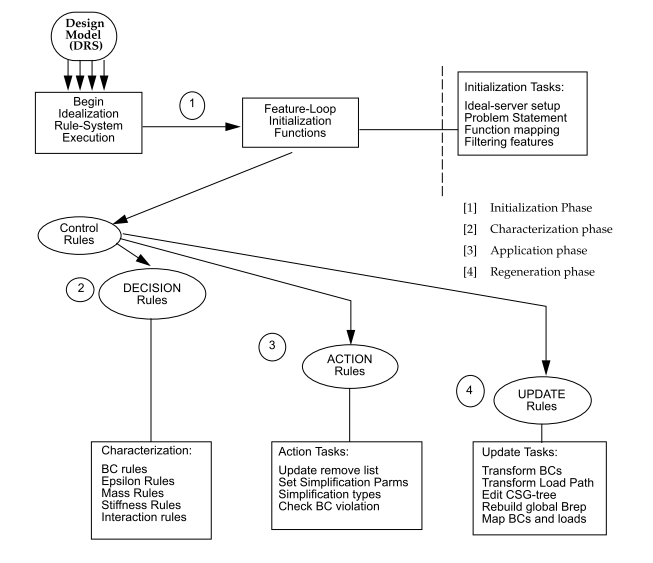
\includegraphics[width=0.5\linewidth]{..//Common/images/DefeaturingDabke.png}
\end{frame}


\begin{frame}{Sang Hung Lee - Korea}
Lee \cite{Lee2005} elaborated a method to reorder design features in the history tree and then to re-execute the history of the reordered features up to the given level of simplification. 

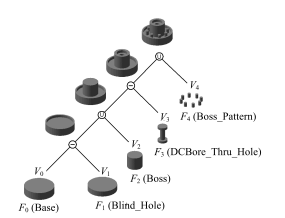
\includegraphics[width=0.5\linewidth]{..//Common/images/DefeaturingSHLeeSmall.png}

\end{frame}

\begin{frame}{Hamdi Mounir}
 Hamdi \cite{Hamdi2005}  seem to test individual features for removal, but approach in this paper takes into account the parent-child relationship between features as well. 

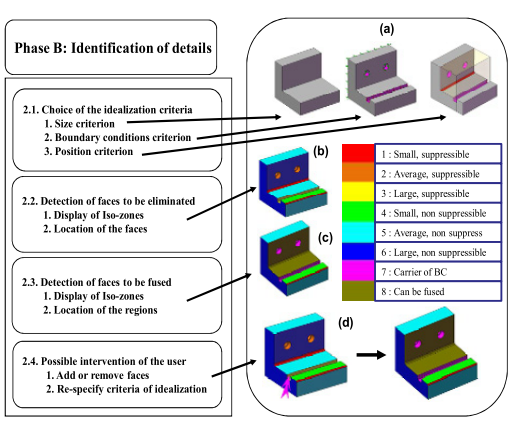
\includegraphics[width=0.5\linewidth]{..//Common/images/DefeaturingHamdi.png}
\end{frame}

\begin{frame}{Danglade 2013}
Danglade\cite{Danglade2013} proposed an approach that uses machine learning techniques to identify rules driving the de-featuring step.

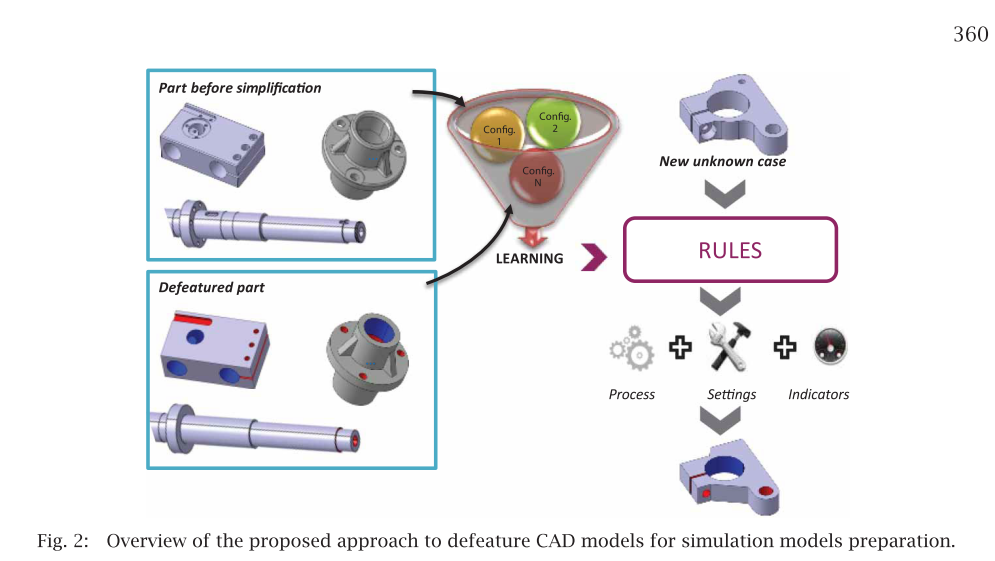
\includegraphics[width=0.7\linewidth]{..//Common/images/DefeaturingDanglade.png}
\end{frame}
